\documentclass[convert]{standalone}

\usepackage{tikz}
\usepackage{standalone}
\usepackage{tikz-feynman}

\usepackage{xcolor}

\begin{document}

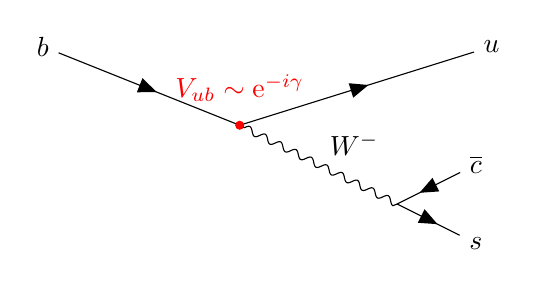
\begin{tikzpicture}
    \begin{feynman}
        \vertex (b) {\(b\)};
        \tikzfeynmanset{every vertex={dot,minimum size=1mm, red}}
        \vertex[dot, below right=1cm and 2.5cm of b] (v1);

        \tikzfeynmanset{every vertex={dot,minimum size=0mm}}
        \vertex[below right=1cm and 2cm of v1] (v2);
        \vertex[right=5.7cm of b] (u) {\(u\)};
        \vertex[above right=0.5cm and 1cm of v2] (cBar) {\(\overline{c}\)};
        \vertex[below right=0.5cm and 1cm of v2] (s) {\(s\)};


        \diagram* { {[edges=fermion]
                (b) -- (v1) -- (u), (cBar) -- (v2) -- (s)},
        (v1) -- [boson, edge label=\(W^-\)] (v2)
        };

        \node[above=0.05cm of v1, label=above:{$\color{red} V_{ub} \sim \mathrm{e}^{-i\gamma}$}] (v3);
    \end{feynman}
\end{tikzpicture}

\end{document}
